\documentclass[a4paper,10pt]{article}
%%%%%%%%%%%%%%%%%%%%%%Paquetes
\usepackage[spanish]{babel}  
\usepackage{indentfirst} %%%%%%%%%%%%%%%%Crear un indent al principio
\usepackage[latin1]{inputenc}%%%%%%%%%%%%� y acentos
\usepackage{tcolorbox}
\usepackage{color}
\usepackage{mathrsfs}
\usepackage{enumerate}
\usepackage{fourier}
\usepackage{latexsym,amsmath,amssymb,amsfonts}
\newcommand{\grad}{\hspace{-2mm}\phantom{a}^{\circ}}


\usepackage[paperwidth=12cm,paperheight=15cm, hmargin={1cm,1cm}, top=1.5cm, bottom=1cm]{geometry}




\pagestyle{empty}


\newenvironment{capitulo}{\begin{tcolorbox}[colback=red!5!white,colframe=red!75!black]}{\end{tcolorbox}}
\newenvironment{ejer}{\begin{tcolorbox}[colback=blue!5,colframe=orange]}{\end{tcolorbox}}
\setlength{\parskip}{2mm}



\author{jltabara@gmail.com}

\title{Calculadora Casio 770 ES}

\date{}





\begin{document}

\begin{capitulo}
\maketitle
\end{capitulo}

\tableofcontents

\newpage


\begin{capitulo}
 \addcontentsline{toc}{subsection}{Operaciones aritm�ticas}
\section*{Operaciones aritm�ticas}
\end{capitulo}



Entrar en el modo adecuado para la realizaci�n de las operaciones aritm�ticas: \textbf{Mode - Comp}.


\begin{ejer}

Realizar las siguientes operaciones:



\begin{itemize}

\item $a)\,2+5, \qquad b)\,5-890 \qquad c)\,345 \times 34 \qquad d)\,(-3) \times 789$

\item $ a)\, 345\div 23\qquad b)\, 34.67\div  4.23 $


\item $ a)\, 2^2 \qquad b)\, 4^3 \qquad c)\, 24.5^{7} \qquad d) \,(-3)^4, \qquad e)\, 3.45^{2.46}$ 

\item $a) \, 4+(3-5)\times 67 +4^5 \qquad b)\, (2+4)^4-7+ 56\div 32$

\item $ \left[2^5\left(4-3^2\right)\right] \div 22.5$

\item $\left[34.78 \cdot \left(2.8-5\right)^2-3+7-89\right]^2$

\end{itemize}

\end{ejer}


\newpage
\begin{capitulo}
 \addcontentsline{toc}{subsection}{Fracciones}
\section*{Fracciones}
\end{capitulo}

\begin{ejer}


\begin{itemize}

\item Simplificar las fracciones:
\[
a)\, \frac{20}{15} \qquad b)\, \frac{13}{5} \qquad c)\, \frac{2345}{8765}
\]

\item Expresar en forma mixta las fracciones anteriores. Tambi�n  como  n�mero decimal 


\item Realizar las operaciones:
\[
a)\, \frac{4}{3} + \frac{7}{3} \qquad b)\, \frac{13}{5}\times\frac{3}{8} \qquad c)\, \frac{6}{7} \div \frac{9}{13}
\]

\item Realizar las operaciones:
\[
 a)\,\left(\frac{4}{5}+ \left(\frac{7}{3} -\frac{4}{5}\right)^2\right) \times 5 - \left(\frac{3}{2}\right)^3
\qquad b)\,\frac{\frac{3}{4} \cdot 8}{\frac{4}{5} +\frac{2}{3}}
\]


\item Hallar la fracci�n generatriz de:
\[
a)\,0.\wideparen{3} \qquad b)\, 45.\wideparen{39} \qquad c)\, 2.67\wideparen{21}\qquad d) 0.\wideparen{3} + \frac{2}{3}
\]

\item Realizar operaciones en el modo \textbf{LineIO}.

\end{itemize}

\end{ejer}


\newpage

\begin{capitulo}
 \addcontentsline{toc}{subsection}{Radicales}
\section*{Radicales}
\end{capitulo}
\enlargethispage{1cm}

\begin{ejer}

\begin{itemize}

\item Calcular las siguientes ra�ces exactas:
\[
a)\, \sqrt{16} \qquad b)\,\sqrt[3]{8} \qquad c) \, \sqrt[5]{32} \qquad  d)\, \sqrt[6]{3^6}
\]


\item Repitir lo anterior sabiendo que $\sqrt[n]{a^m}= a^{m/n}$.

\item Calcular las ra�ces (o potencias):
\[
a)\, 32^{3/4} \qquad b) \, 4^{-1} \qquad c)\, 23.78^{-2/5} \qquad d)\, 34.1^{4.32}
\]

\item Realizar la siguiente operaci�n combinada.
\[
\sqrt{5} +6 \times \sqrt[5]{9}
\]

\item Extraer factores de los radicales cuadr�ticos (\textbf{MathIO}):
\[
a)\,\sqrt{8}  \qquad b) \,  \sqrt{243} \qquad c)\, \sqrt{\frac{8}{243}}
\]


\item Simplificar las operaciones con radicales:
\[
a)3\sqrt{20}- 7\sqrt{5} \qquad b)\, \sqrt{2}\sqrt{8} \qquad c)\, \sqrt{3}\sqrt{8}
\]


\item Racionalizar:
\[
a) \frac{3}{\sqrt{2}} \qquad b)\, \frac{2}{2+\sqrt{5}} \qquad c) \, \frac{6}{\sqrt{6}-\sqrt{2}}
\]



\end{itemize}

\end{ejer}


\newpage

\begin{capitulo}
 \addcontentsline{toc}{subsection}{Exponenciales y logaritmos}
\section*{Exponenciales y logaritmos}
\end{capitulo}

\begin{ejer}

\begin{itemize}

\item Calcula las exponenciales:
\[
a)\, e^1 \qquad b)\, e^5 \qquad c)\, e^{4.61} +3\times e^{\frac{8}{3}}
\]

\item Calcula los siguientes logaritmos neperianos:
\[
a)\,\ln(e) \qquad b)\ \ln\left(e^7\right) \qquad c)\,\ln(56.3) + 12^{5.1}
\]


\item Calcula los siguientes logaritmos decimales:
\[
a)\, \log(1000) \quad b)\, \log(-3) \quad c)\, \log(3.21) \quad d)\,\log(321)
\]

\item Calcula los siguientes logaritmos:
\[
a)\, \log_2(32) \quad b)\, \log_3(81) \quad c)\,\log_{\sqrt{2}} (4) \quad d)\, \log_{3}\left(\sqrt[4]{3^5}\right)
\]

\item Comprueba la f�rmula de cambio de base:
\[
a)\log_{5.2}(8.9) \qquad b)\, \log_{2}(89)
\]

\item Comprueba propiedades de los logaritmos:
\[
a)\,\log(34 \cdot 56)\qquad b)\, \log\left(\frac{789}{34}\right) \qquad c)\ \log\left(56^4\right)
\]
 


\end{itemize}



\end{ejer}





\newpage

\begin{capitulo}
 \addcontentsline{toc}{subsection}{Trigonometr�a}
\section*{Trigonometr�a}
\end{capitulo}

\enlargethispage{1cm}

\begin{ejer}


\begin{itemize}

\item Transforma los siguientes n�meros a notaci�n sexadecimal:
\[
a)\, 3.5 \qquad  b)\, 4.99 \qquad c) \, -8.923
\]

\item Realiza las siguientes operaciones sexadecimales:
\[
a)\, 4\grad 5' 34'' + 56\grad 2'45'' \qquad b) \, 4\times(3\grad 2')-2\grad 0'57''
\]

\item Convertir en radianes y grados los siguientes �ngulos: 
\[
a)\, 30^0 \qquad b)\, 20^0 \qquad c)\, \frac{5\pi}{3} \qquad d)\, \frac{13\pi}{6}
\]


\item Razones trigonom�tricas en grados y radianes.
\[
a)\sin(60) \qquad b)\, \cos(78) \qquad c)\, \sin\left(\frac{\pi}{3}\right)\qquad d)\,\tan\left(\frac{13\pi}{6}\right)
\]


\item Funciones trigonom�tricas inversas.
\[
a)\, \arcsin\left(\frac{\sqrt{2}}{2}\right)\qquad \arctan(\sqrt{3}) \qquad c)\mathrm{arccos}(0.345)
\]

\item Funciones hiperb�licas.
\[
a)\,\sinh(3) \qquad b)\, \tanh\left(\frac{8}{9}\right) \qquad c)\,\mathrm{arccosh}(4)
\]

\end{itemize}

\end{ejer}

\newpage

\begin{capitulo}
 \addcontentsline{toc}{subsection}{Funciones y ecuaciones}
\section*{Funciones y ecuaciones}
\end{capitulo}


\begin{ejer}
\begin{itemize}
\item Calcular distintos valores num�ricos de las funciones:
\[
f(x)=-0.2 x^3+\sin(x+2)+x
\]
\[
g(x,y)= 3x+\sin(y)
\]

\item Construye una tabla para la funci�n:
\[
f(x)=-0.2 x^3+\sin(x+2)+x
\]

\item Resuelve  la ecuaci�n anterior igualada a cero.
\begin{center}
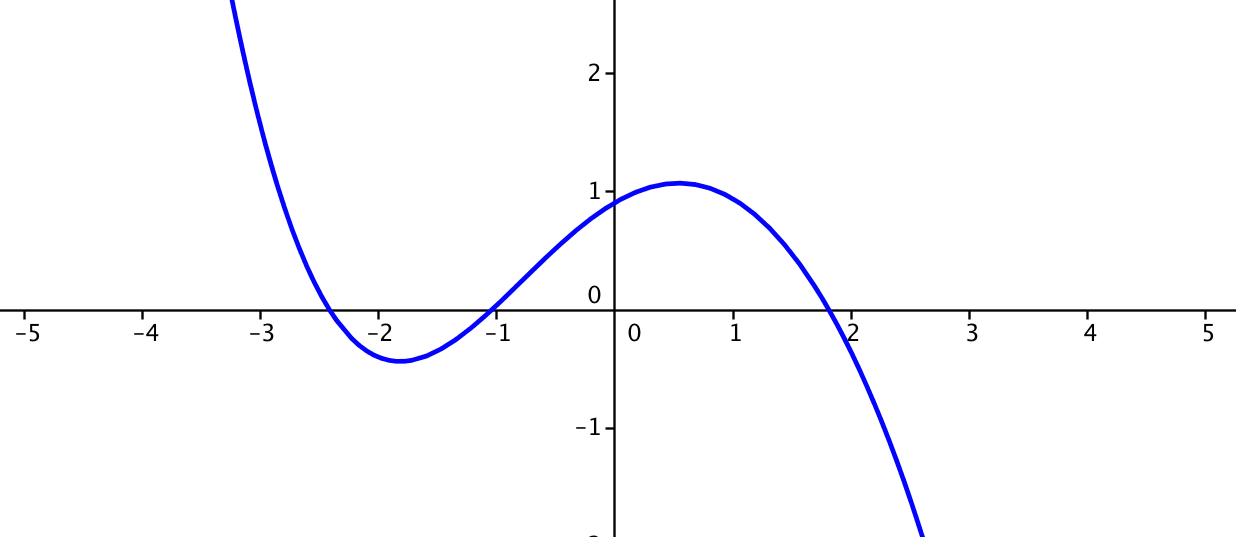
\includegraphics[scale=0.75]{funcion.png} 
\end{center}

\end{itemize}


\end{ejer}



\newpage

\begin{capitulo}
 \addcontentsline{toc}{subsection}{Ecuaciones de segundo y tercer grado}
\section*{Ecuaciones de segundo y tercer grado}
\end{capitulo}


\begin{ejer}
\begin{itemize}
\item Resuelve las ecuaciones de segundo grado.

\begin{tabular}{ll}
 a)\, $x^2-5x+6=0$ & b)\, $x^2+2x+1=0$  \\
  & \\
 c)\, $x^2+1=0$ & d)\, $x^2-4x+13=0$   \\
  & \\
 e)\, $6.4x^2+7.34x+7.11=0$ &   
\end{tabular}

\item Resolver las ecuaciones de tercer grado:

\begin{tabular}{l}
a)\,$ x^3-6 x^2+11 x-6=0$\\
 \\
b)\,$ x^3-3 x^2+x-3=0$\\
\\
c)\, $x^3-5 x^2+7 x-3=0$ \\
\\
d)\, $x^3-6 x^2+21 x-26=0$\\
\\
e)\, $3.1x^3+5.23x+9=0$
\end{tabular}



\end{itemize}


\end{ejer}

\newpage

\begin{capitulo}
 \addcontentsline{toc}{subsection}{Sistemas de ecuaciones}
\section*{Sistemas de ecuaciones}
\end{capitulo}

\begin{ejer}

Resuelve los siguientes sistemas de ecuaciones:
\[
\begin{cases}
3x + 4y &=11\\
2x - 7y & = -12
\end{cases}
\]
\[
\begin{cases}
3.7x + \sqrt{45}y &=1\\
\displaystyle 13x-67y& = \frac{3}{4}
\end{cases}
\]

\[
\begin{cases}
3x + 4y &=11\\
3x + 4y & = 12
\end{cases}
\]

\[
\begin{cases}
3x + 4y +5z  &=1\\
2x - 7y  +5z & = 2\\
-4 x +9y & = 3
\end{cases}
\]




\end{ejer}



\newpage


\begin{capitulo}
 \addcontentsline{toc}{subsection}{N�meros complejos}
\section*{N�meros complejos}
\end{capitulo}

\enlargethispage{1cm}
\begin{ejer}

\begin{itemize}

\item Realiza las siguientes operaciones con complejos:

\[
a)\,  (3+5i) + (4+8i) \qquad b)\, (2-3i)\cdot (2-i)
\]
\[\displaystyle a)\, \frac{2+7.6i}{2+8i}\qquad b)\, i^9\qquad c)\, \sqrt{-1}
\]



\item Calcula el m�dulo y el argumento de:
 
\[
a)\, 4i \qquad b)\,  6-2i \qquad c) \, (2-3i)^3
\]
 

 
\item Transforma en bin�mica los n�meros:
 
\[
 a) \, 1_{90} \qquad b)\, 6_{45} \qquad c)\, 45.89_{23.8}
 \]



\item Realiza las operaciones en forma polar:

\[
a)\, 2_{30} \cdot 5_{70}\qquad b)\, (3_{20})^3
\]


\item Calcula el conjugado de:
\[
a)\, 3+4i \qquad b)\, 4_{30}
\]

\item Utilizar las teclas \textbf{Pol} y \textbf{Rect} para cambiar de forma bin�mica a polar y viceversa los n�meros:
\[
a) \, 3+4i \qquad b) \, 4_{30}
\]

\end{itemize}

\end{ejer}




\newpage

\begin{capitulo}
 \addcontentsline{toc}{subsection}{Combinatoria}
\section*{Combinatoria}
\end{capitulo}

\begin{itemize}
\item Operaciones con factoriales.
\[
a)\, 5! \qquad b)\, 70! \qquad c)\, \frac{10!}{3! \cdot  5!}
\]

\item Operaciones con variaciones (sin repetici�n).
\[
a)\, \mathrm{V\,}_{23}^5\qquad b)\,\mathrm{V\,}_{10}^3  \qquad c)\, \frac{10!}{7!} \qquad d)\, \mathrm{V\,}_{12}^{12}
\]
\item Operaciones con combinaciones.
\[
a)\,\mathrm{C\,}_{10}^3\qquad b)\,\mathrm{C\,}_{10}^7\qquad c)\, \frac{10!}{7!\cdot 3!}\qquad  d)\,\mathrm{C\,}_{100}^1
\]


\item Genera distintos tipos de n�meros aleatorios.

\item Generar una tabla de n�meros aleatorios.

\end{itemize}

\newpage

\begin{capitulo}
 \addcontentsline{toc}{subsection}{Vectores}
\section*{Vectores}
\end{capitulo}




\begin{ejer}

Dados los vectores $u=(3,2,1)$ y $v=(-6,1,9)$.

\begin{itemize}

 
\item Calcular las combinaciones lineales:
\[
 a) \, u+v  \qquad b)\,    u-v  \qquad c)\, 4u+7v 
 \]

\item Calacular los productos escalares:
\[
a)\, u\cdot v \qquad b)\, u\cdot u \qquad c) \,|u|
\]

\item Calcular los productos vectoriales:
\[
a)\, u \times v  \qquad b) \, v\times u \qquad c)\, u\times u
\]

\item Comprobar que el siguiente resultado es nulo:
\[
(u\times v)\cdot u
\]

\item Calcular el vector unitario de $u$ y el �ngulo que forman los vectores $u$ y $v$.


\end{itemize}

\end{ejer}


\newpage

\begin{capitulo}
 \addcontentsline{toc}{subsection}{Matrices}
\section*{Matrices}
\end{capitulo}

\begin{ejer}

Dadas las matrices:
\[
A=\begin{pmatrix}
2 & 3\\
5 & -1
\end{pmatrix} \qquad 
B =
\begin{pmatrix}
8 & -3\\
5 & 9
\end{pmatrix}
\]

\begin{itemize}

\item Calcular las combinaciones lineales:
\[
a)\, A+B\qquad  b)\, A-B\qquad c)\, 4A-7 B
\]

\item Calcular los siguientes productos:
\[
a)\,  A\cdot B \qquad   b)\, B \cdot A  \qquad c)\, A \cdot B \cdot A
\]

\item Calcular las siguientes potencias:
\[
  a)\, A^2 \qquad   b)\, A^3 \qquad  c)\, A^4 
  \]
  
 \item Realizar las operaciones:
 \[
 a)\, \mathrm{det}(A) \qquad  b)\,  A^t  \qquad  c) \, A^{-1}
 \]

\item Realizar las operaciones:
\[
  a)\, A^{-1} \cdot A \qquad   b)\, (A^{-1})^t\qquad c)\,(A^t)^{-1}
  \]


\end{itemize}


\newpage

\end{ejer}\begin{capitulo}
 \addcontentsline{toc}{subsection}{Otras bases de numeraci�n}
\section*{Otras bases de numeraci�n}
\end{capitulo}

\begin{ejer}

\begin{itemize}

\item Convertir el n�mero 456  a distintas bases de numeraci�n.

\item Convertir $2AF_{16}$ a distintas bases.

\item Convertir $10101011_2$ a distintas bases.

\item Realizar la operaci�n:
\[
1010_2 + AF_{16} \cdot 34_{10}
\]

\item Comprobar la tabla de verdad de la operaci�n \textbf{and}.

\item Realizar la operaciones:
\[
a)\,1010 \mathrm{\ or\ } 1100 \qquad b)\,1010 \mathrm{\ xor\ } 1100 \qquad c)\,10 \mathrm{\ xor\ } 12
\]

\item Realizar las operaciones:
\[
a)\, \mathrm{\ not \ } 101110 \qquad b)\, -56
\]

\end{itemize}

\end{ejer}







\newpage

\begin{capitulo}
 \addcontentsline{toc}{subsection}{Estad�stica unidimensional}
\section*{Estad�stica unidimensional}
\end{capitulo}

\begin{ejer}

Dada la tabla de frecuencias:
\begin{center}
\begin{tabular}{c|c}
x & f \\ \hline
3 & 4 \\
4 & 7 \\
6 & 5
\end{tabular}
\end{center}
calcula:

\begin{itemize}

\item Calcula la suma de los datos y la suma de los cuadrados de los datos.

\item Calcula el n�mero de datos, la media, la desviaci�n t�pica y la varianza.

\item Calcula el m�nimo y el m�ximo de los datos.

\item Dado una normal tipificada $X$ calcula:
\[
a)\, \mathrm{P}[X <1.2] \qquad b)\, \mathrm{P}[0<X<1.2] \qquad c)\, \mathrm{P}[X >1.2]
\]
\begin{center}
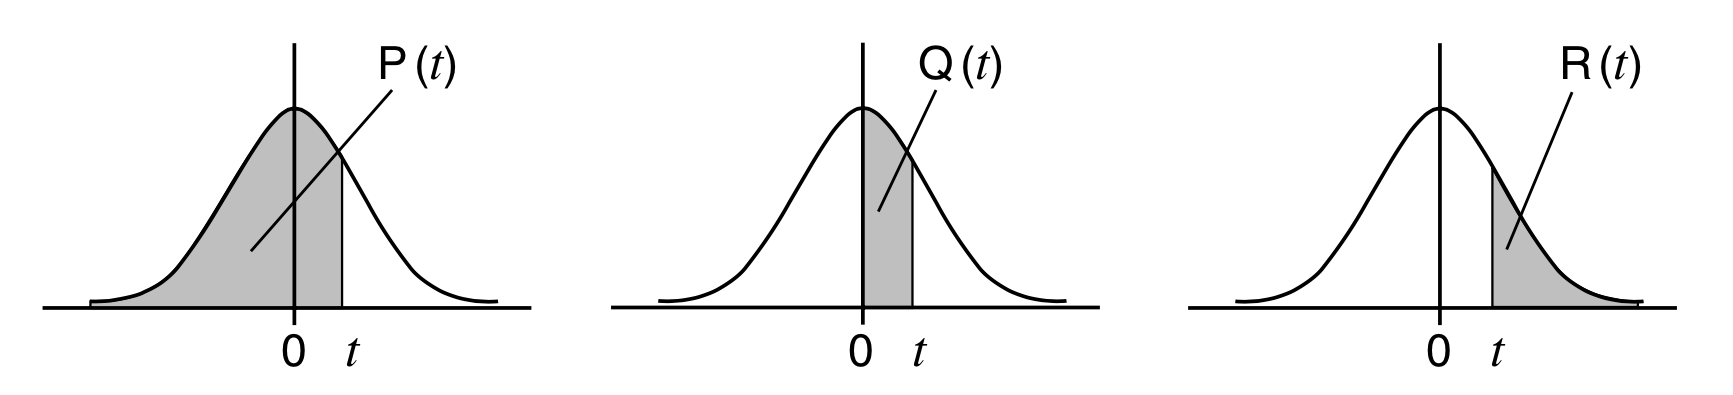
\includegraphics[scale=0.12]{distribucion.png} 
\end{center}

\end{itemize}

\end{ejer}

\newpage

\begin{capitulo}
 \addcontentsline{toc}{subsection}{Estad�stica bidimensional}
\section*{Estad�stica bidimensional}
\end{capitulo}




\newpage



sumar los 100 primeros numeros naturales

sumar las 64 primeras potencias de 2

sumar 1/x2 y valor de pi2/6




\end{document}



